%        File: main.tex
%     Created: Wed Oct 22 06:00 PM 2008 E
% Last Change: Wed Oct 22 06:00 PM 2008 E
%
\documentclass[a4paper,12pt]{article}

\usepackage{setspace}
\usepackage{cite}
\usepackage{graphicx}
\usepackage{amsmath}
\usepackage{amssymb}
\usepackage{url}

\author{Kefei Lu}
\title{Project II Report:\\Internet Traffic Classification Using Naive Bayesian Analysis}

\doublespacing
\begin{document}
\maketitle
\tableofcontents
\newpage

\section{Introduction}
The internet traffic identification plays an important role in network management. It enables network operators to better predict future network metrics and demands, security personnel to detect network anomalous behaviour, researchers to improve network performance.

% Many traffic analysis researches are based on data mining techniques. For example, T. Auld, et al. proposed a traffic classifier that can achieve high accuracy throughout a range of web application types without any source or destination host address or port information \cite{auld2007bnn}. The supervised machine learning based on Bayesian trained neural network is used in their approach. An advantage of their approach is providing classification without access to the packet contents. This powerful advantage ensures the wide application of the approach in network traffic analysis. 

This project is based on the work of Moore et al \cite{moore2005itc}. They applied a Naive Bayes estimator to categorize traffic by application. Uniquely, their work capitalized on hand-classified network data, using it as input to a supervised Naive Bayes estimator. It was indicated that with the simplest of Naive Bayes estimator they were able to achieve about 65\% accuracy on per-flow classification and with powerful refinements they could improve this value to between than 95\%.

In this project, a simple internet traffic supervised classification system based on the Naive Bayes method \cite{moore2005itc} is implemented using C++ programming language with C standard library and C++ standard template library (STL). A dataset system and a classifier system is implemented. They are built to be modularized and can be easily extended, thanks to the object oriented feature of C++. More details will be presented in Section \ref{sec:imp}.

Additionally, some utility applications are developed to help make preprocessing more efficiently. For example, \verb|grab_inst| grabs all instances lines from an ARFF file, prints them to standard output, throwing out other things. \verb|port_hist| prints the histogram of the port numbers of flows belonging to a certain class in an ARFF file. \verb|reindex| renames the attribute names to increasing integer numbers.

For detailed information, please refer to the project reference manual.

\subsection{Program Usage}
The program is developed on Linux using G++ version 4.2.4. Only C standard libraries and C++ STL are used so that the program should be portable to any other platforms. It has been tested on Ubuntu 8.04.1 with G++ 4.2.4 and Microsoft Windows XP with Visual C++. But it is recommended to compile and run the program under Linux/Unix environments with GNU Automake tools \cite{automake}.

To build the project, type \verb|make| in shell command line. To clean up the build, type \verb|make clean|. 

After successful compilation, link the local file \verb|test.arff| against the real arff file, say \verb|data/test.arff.small|, the command is 

\begin{verbatim}
ln -sf data/test.arff.small test.arff
\end{verbatim}

Note that since the datasets are too large, in the distributed package of this program, only a sample arff file \verb|test.arff.small| is placed in \verb|data\| directory. For other datasets, refer to \cite{moore_website}.

Also note that since the sample dataset is combined manually from many datasets, it may NOT have a normal performance when classifying on it.

The following sample codes illustrates how to use the program.
\singlespacing
\begin{verbatim}
#include "common.h" // normally included headers
#include <iostream>
#include "dataset.h" // Dataset class
#include "classifier.h" // classifier classes
#include "xvalidator.h" // cross validation

using namespace std;

int main()
{
    // initiate a dataset using test.arff
    Dataset dataset("test.arff"); 

    // Initiate a naive Bayes classifier based on dataset
    NaiveBayesClassifier c(dataset,248);

    // train using WHOLE dataset
    // One can also specify the training inst. using
    // train_set() method.
    c.train();

    // test over WHOLE dataset
    // One can also specify the training inst. using
    // test_set() method.
    c.test();

    // No need to use train() test() directly.
    // Just use cross validator!
    Xvalidator x(&c);
    // set seed
    x.seed() = 3;
    // set fold
    x.fold() = 8;
    // Start! That's that easy!
    x.xvalidate();
    
    return 0;
}
\end{verbatim}
\doublespacing

\subsection{The Documentation}
The project also comes with a complete and detailed manual, documenting the whole source files. The document is based on a special c++ comment style in the source file, and is generated using the open source documentation tool \verb|Doxygen| \cite{doxygen}. To build the documents, pleae make sure to have a working Doxygen, then type \verb|make doc|, and the manual is availabe in directory \verb|doc/|. 

The document comes in two formats, the html format is located in \verb|doc/html|, and is ready for use. The pdf format is in \verb|doc/latex|, before using, please \verb|cd| into the directory, and type \verb|make|.

The pdf format of the manual should have been submitted together with this report.

\section{The Algorithms: Naive Bayes Method}
\label{sec:alg}
%\subsection{The Basic Naive Bayes Method}
The naive Bayes classifier uses naive Bayes method in classification. It is based on the criteria that one wishes to choose a class label $i$ for a given instance (observation) $\mathbf{o}=\{a_1,a_2,\ldots,a_M\}$, such that the probability $Pr(c_i|\mathbf{o})$ is maximized. In the above equation, $M$ is the number of attributes that the instance has. This criteria is called Maximum A Posteriori (MAP) criteria. Mathematically, it is written as:
\begin{equation}
    \label{eq:map}
    i = argmax_{i \in \mathbf{I}} {Pr(c_i|\mathbf{o})},
\end{equation}
where $\mathbf{I}$ is the set of all possible values of $i$.

In the sense of naive Bayes method, the a posteriori probability in Eq. \ref{eq:map} can be further written as:
\begin{align}
    Pr(c_i|\mathbf{o}) & = \frac{Pr(\mathbf{o}|c_i)Pr(c_i)}{Pr(\mathbf{o})} \\
    & = \frac{ Pr(c_i) \prod_{k=0}^{M} { Pr(a_k|c_i) } } { \sum_{j=0}^{N} {Pr(c_i) \prod_{k=0}^{M}{Pr(a_k|c_j)} }},
\end{align}
where we assume that the attributes consisting of the observation are independently distributed.

To estimate the conditional probabilities, the naive Bayes method further assumes that random variables $\{A_k|c_j\}$ are normally distributed.

Therefore, it is able to evaluate a posteriori probabilities for all class indices. The classification is made on the class with largest a posteriori probability.

% \subsection{The Naive Bayes Method With Kernel Estimation}
\section{The Project Structure}
\begin{figure}[tbp]
    \centering
    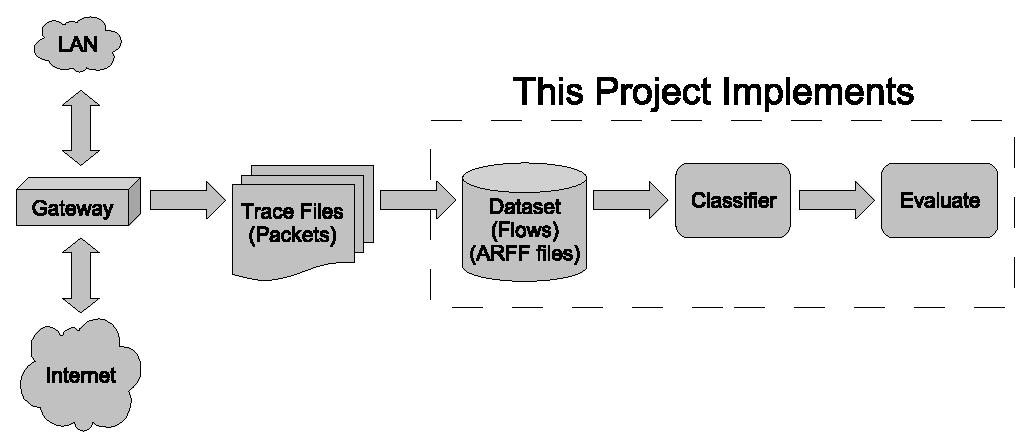
\includegraphics[width=1.1\textwidth]{pic/flow_chart.eps}
    \caption{The flow chart of network traffic classification.}
    \label{fig:flow_chart}
\end{figure} 

As shown in Figure \ref{fig:flow_chart}, the network flow classification process consists of several procedures. A network device records network trace files from the internet. The trace files are then processed during which packet header information are processed and network flows are identified. The flows are recorded in ARFF format to form the desired dataset. The dataset is then feed into the naive Bayes classifier to train the model, then test and evaluate the performance.

It is worth mentioning that it is not trivial to identify flows from packet header traces. Since for this particular project, the authors of \cite{moore2005itc} provides ARFF flow dataset at \cite{moore_website}, I will not focus on the procedure of obtaining traces and identifying flows from packets. For detailed information, please refer to \cite{moore2005duf}.

\section{The Implementation}
\label{sec:imp}
\begin{figure}[tbp]
    \centering
    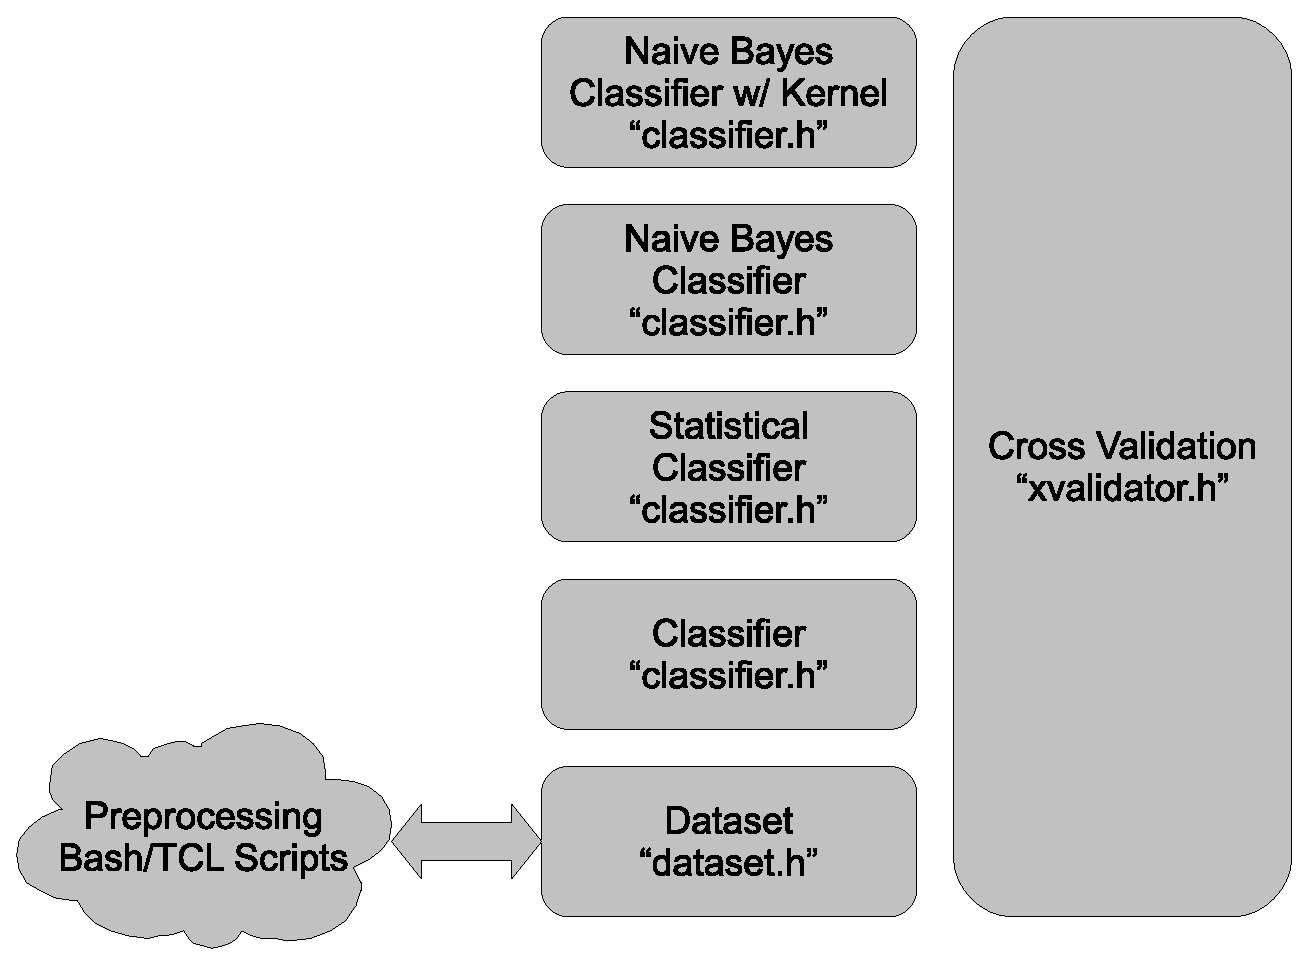
\includegraphics[width=0.9\textwidth]{pic/struct.eps}
    \caption{The structure of the implementation.}
    \label{fig:struct}
\end{figure} 
Once given the algorithm as described in Section \ref{sec:alg}, the implementation is straightforward. However, to make the implementation general and extendible is not trivial.

The implemented project consists of several parts as shown in Figure \ref{fig:struct}.

First of all, a complete, full functioning data set system is implemented. The data set system is able to load ARFF files as the WEKA system does. It is able to take as many as $2^{64}-1$ instances, each consists of as many as $2^{64}-1$ attributes. The data set system is able to take numeric attributes and nominal attributes, and is able to be extended to add other attribute types. 

Manipulating on the data set system, the naive Bayes classification (NBC) system is implemented. It is able to test and train on a given data set, with specified parameters as the testing instances, training instances, etc. The classifiers are written in a way that they can be easily extended to other classifiers. 

For example, the basic classifier class specifies the interface that a classifier should implement, i.e., classifies an instance. Then statistical classifiers implement this interface by using the maximum a posteriori (MAP) criteria. Then the naive Bayes classifier inherits from the statistical classifier by calculating the a posteriori probability assuming that attributes are independent and normally distributed conditioned on a given class. Similarly, the naive Bayes classifier with kernel estimation (NBCKE) inherits from the basic naive Bayes classifier, only having different method to calculate the conditional probability of an attribute. 

In this way, future classifiers can be easily implemented based on existing ones. In this project, the basic classifier (abstract), statistical classifier (abstract), and the naive Bayes classifier are implemented. The naive Bayes classifier with kernel estimation is left for future implementing.

Besides, the cross validation class is implemented to manipulate the classifier class. It splits the dataset into n folds, using only one fold for testing and the rest for training. This process is iterated for n times over the n folds. And the performance is averaged. The cross validation can be stated as following:

\singlespacing
\begin{verbatim}
randomize seed 
split dataset into folds
for each fold i:
    train dataset - fold i 
    test fold i
    store performance i 
average on performance
\end{verbatim}
\doublespacing

\section{The Result}
\label{sec:result}
To verify the work of this project, 8-fold cross validation is conducted on the 9 datasets, each cross validation is randomized 5 times. Then the performances are averaged to produce the following results.

In the following results, the accuracy is defined as the total number of correctly classified instance diveded by total number of instances. The trust is defined as the probability that an instance belongs to a certain class given that it has been classified as this class. The trust indicates how much one can believe the classification.

\singlespacing
\begin{verbatim}
Naive Bayes Accuracy: 62.19%
Moore et al Accuracy: 65.26%
\end{verbatim}

\begin{verbatim}
Naive Bayes Trust, Moore et al. Trust
WWW 	96.7%			98.31%
MAIL	71.2%			90.69%
BULK	66.32%			53.77
SERV	68.9%			35.92%
DB	47.5%			61.78%
P2P	2.8%			4.96%
ATTACK	0.898%			1.10%
MMEDIA	56.5%			32.30%
\end{verbatim}
\doublespacing

\begin{table} 
\begin{tabular}[tbp]{c c c c c c c c c c c c c}
54.3 & 43.5 &  0.5 &  1.7 &  0.0 &  1.6&   1.2&   3.7&   2.5&   0.2 &  0.1 &  0.0 \\
0.0 & 273.6 &  0.1 &  0.0 &  0.0 &  0.0&   0.0&   0.0&   0.0&   0.1 &  0.0 &  0.0 \\
0.0 &  0.0  &11.7  & 0.0  & 0.0  & 0.0 &  0.0 &  0.0 &  0.0 &  0.0  & 0.0  & 0.0  \\
0.2 &  0.0  & 0.0  &41.2  & 0.0  & 0.0 &  0.0 &  0.1 &  0.0 &  0.0  & 0.0  & 0.0  \\
1.6 & 10.2  & 0.0  & 0.0  & 1.8  & 5.7 &  0.1 &  0.0 &  1.2 &  0.1  & 0.0  & 0.0  \\
3.6 & 13.3  & 0.1  & 0.0  & 0.0  & 4.3 &  0.0 &  0.3 &  0.1 &  0.1  & 0.0  & 0.0  \\
0.0 &  0.0  & 0.0  & 0.0  & 0.0  & 0.0 & 39.7 &  0.0 &  0.0 &  0.0  & 0.0  & 0.0  \\
0.0 &  0.0  & 0.0  & 0.0  & 0.0  & 0.0 &  0.0 &152.8 &  0.0 &  0.0  & 0.0  & 0.0  \\
0.0 &  0.0  & 0.0  & 0.0  & 0.5  & 0.0 &  0.0 &  0.0 & 14.8 &  0.0  & 0.0  & 0.1  \\
0.0 &  0.0  & 0.0  & 0.0  & 0.0  & 0.0 &  0.0 &  0.0 &  0.0 & 26.8  & 0.0  & 0.0  \\
0.0 &  0.0  & 0.0  & 0.0  & 0.0  & 0.0 &  0.0 &  0.0 &  0.0 &  0.0  & 0.1  & 0.0  \\
0.0 &  0.0  & 0.0  & 0.0  & 0.0  & 0.0 &  0.0 &  0.0 &  0.0 &  0.0  & 0.0  & 0.0  \\
\end{tabular}
\caption{An Example of A Confusion Matrix.}
\end{table}

The implemented work can also provide the confusion matrix. However since average across different cross validations is not provided, I only present the confusion matrix of 8-fold cross validation on dataset \verb|entry02.weka.allclass.arff| using seed 2 as following.

It can be seen from the result that the performance is close to that of the original work by Moore et al. However, there is some difference between the two performances. Note that this is mainly because of the different use on the datasets but rather than the algorithm itself.

\subsection{Feature Selection and Dimension Reduction}
Authors of \cite{moore2005itc} also proposed a method to select good features. The method used is Fast Correlation-Based Filter (FCBF). At the end of the paper, the authors identified several good features using FCBF. In this project, classifications are done using only these good features. It is shown that feature selection gives great improvement on classification performances. Due to time limit, this experiment is only conducted using dataset \verb|data/entry01.weka.allclass.arff| using cross validation. The results are shown as below. 

Since these haven't been randomized over seeds and over different datasets, it's not reasonable to compare with the work in \cite{moore2005itc}.

\singlespacing
\begin{verbatim}
Naive Bayes Accuracy with FCBF: 94.29%
\end{verbatim}

\begin{verbatim}
Naive Bayes Trust with FCBF
WWW 	98.7%	 
MAIL	90.4%	 
BULK	52.97%	 
SERV	97.39%	 
DB	100.0%	 
P2P	6.42%	 
ATTACK	9.72%	 
MMEDIA	21.72%	 
\end{verbatim}
\doublespacing

\bibliographystyle{IEEEtran}
\bibliography{data_mining}

\end{document}

